\documentclass[main.tex]{subfiles}

\begin{document}
\section{Methodology} \label{methodology}

In this section we describe the techniques we considered and brainstormed during the project and those that are implemented in the base model.

\begin{center}
  \begin{table}[!htp]
    \centering
    \caption{Summary of techniques used for each tasks}
    \begin{tabular}{*4c}
      \toprule
      Task            & Subtask      & Techniques &     Base Model \\
      \midrule
      Image Processing & {} & {} & {} \\
      \hline
      Feature Extraction  & Global Descriptors & asd &\checkmark \\
      \hline
      {} & {}             & Hu's Invariant moments & \checkmark \\
      \hline
      {} & {}             & Complex moments & \checkmark \\
      \hline
      Classification & {} & Multivarate Gaussian Model & \checkmark \\
      {}             & {} & Linear Discriminant \\
      \bottomrule
    \end{tabular}
  \end{table}
\end{center}

\subsubsection*{Background Subtraction}
In this coursework, since a background image is not readily available, we have to model it. Noting that images varies in illumination, we have to make the images comparable by normalising it first, using the following formula.
$$ P_{r,c}(R',G',B')=(\frac{R}{\sqrt(R^2+G^2+B^2)},\frac{G}{\sqrt(R^2+G^2+B^2)},\frac{B}{\sqrt(R^2+G^2+B^2)})$$

With objects scattered around randomly in the images, we find the median of all image pixels for each channel separately in order to reconstruct the background.

The outcome of the background with and without normalisation is shown in \autoref{bg_model}.

\begin{figure}[!h]
  \centering
  \begin{subfigure}[b]{.45\textwidth}
    \centering
    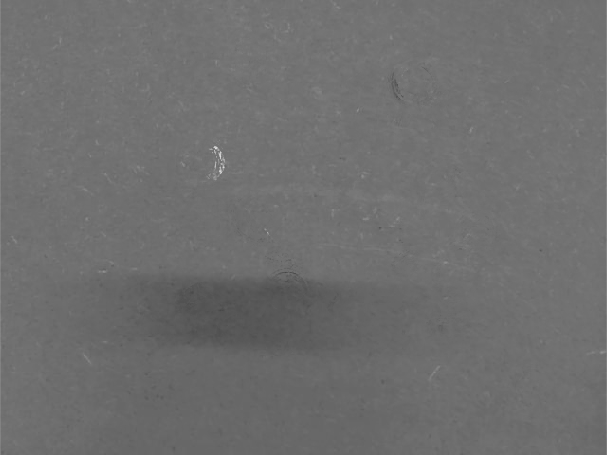
\includegraphics[width=\textwidth]{./img/bg_model/org_1.png}
    \caption{Background model without normalisation}
  \end{subfigure}
  \begin{subfigure}[b]{.45\textwidth}
    \centering
    
\includegraphics[width=\textwidth]{./img/bg_model/norm_1.png}
    \caption{Background model after normalisation}
  \end{subfigure}
  \caption{Background model generated from all 14 images}
  \label{bg_model}
\end{figure}


% Our approach is similar, but uses a neighbourhood of pixels around a target point. Hence, for a window of size 3, we have
% $bg\_model_{r,c} = median(i_{r+1,c+1}, i_{r+1,c}, i_{r+1,c-1},
%                           i_{r,c+1}, i_{r,c}, i_{r,c-1},
%                           i_{r-1,c+1}, i_{r-1,c}, i_{r-1,c-1}) $.
%
% The outcome of the background (with and without normalisation) are:
%
% \begin{figure}[!h]
%   \centering
%   \begin{subfigure}[t]{\textwidth}
%     \centering
%     \begin{subfigure}[t]{.3\textwidth} %% taking median
%         \centering
%         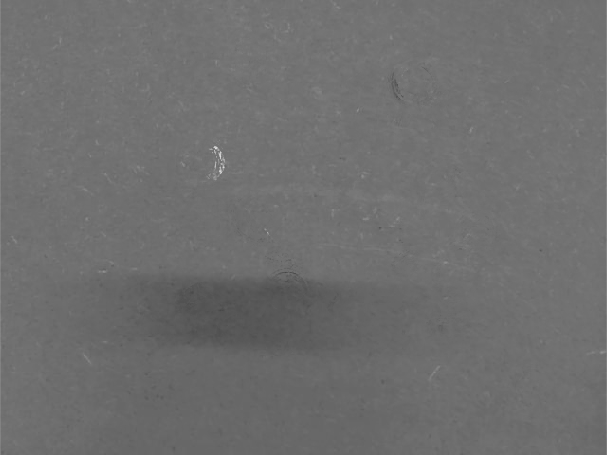
\includegraphics[width=\textwidth]{./img/bg_model/org_1.png}
%     \end{subfigure}
%     \begin{subfigure}[t]{.3\textwidth} %% window_size = 3
%         \centering
%         
\includegraphics[width=\textwidth]{./img/bg_model/org_3.png}
%     \end{subfigure}
%     \begin{subfigure}[t]{.3\textwidth} %% window_size = 5
%         \centering
%         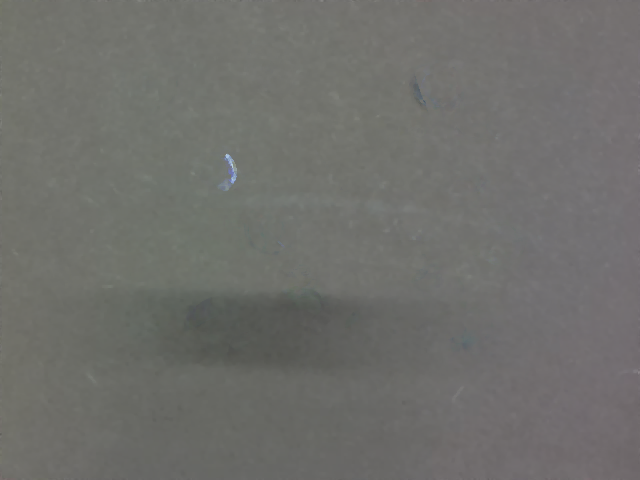
\includegraphics[width=\textwidth]{./img/bg_model/org_5.png}
%     \end{subfigure}
%   \end{subfigure} %% LOWER IMAGE - NORMALISED
%   \begin{subfigure}[b]{\textwidth}
%     \centering
%     \begin{subfigure}[t]{.3\textwidth} %% taking median
%         \centering
%         
\includegraphics[width=\textwidth]{./img/bg_model/norm_1.png}
%         \caption{Neighbouhood=1}
%     \end{subfigure}
%     \begin{subfigure}[t]{.3\textwidth} %% window_size = 3
%         \centering
%         
\includegraphics[width=\textwidth]{./img/bg_model/norm_3.png}
%         \caption{Neighbourhood=3}
%     \end{subfigure}
%     \begin{subfigure}[t]{.3\textwidth} %% window_size = 5
%         \centering
%         
\includegraphics[width=\textwidth]{./img/bg_model/norm_5.png}
%         \caption{Neighbourhood=5}
%     \end{subfigure}
%   \end{subfigure}
%   \caption{Sample images from given data.}
%   \label{montage_bg}
% \end{figure}


The sample images with their background removed is shown in \autoref{montage_data_bgremove}. It is evident that the background removal process removed the background - making the images appearing black. However, it also inevitably reduce the intensity for the bottom half of each images, such that the objects are no longer salient to our eyes. This is because the background we modelled have a lower intensity at the bottom, possibly due to presence of shadow in all 14 images.

Nevertheless, the historgram  is still bimodal, which is essential for thresholding to be effective.

\subsubsection*{Segmentation}



\subsection{Classification}





\end{document}
